% Copyright 2004 by Till Tantau <tantau@users.sourceforge.net>.
%
% In principle, this file can be redistributed and/or modified under
% the terms of the GNU Public License, version 2.
%
% However, this file is supposed to be a template to be modified
% for your own needs. For this reason, if you use this file as a
% template and not specifically distribute it as part of a another
% package/program, I grant the extra permission to freely copy and
% modify this file as you see fit and even to delete this copyright
% notice. 

\documentclass[xcolor=table]{beamer}
\usepackage{menukeys}[os=win]
\usepackage{textcomp}
\usepackage{tcolorbox}
\usepackage{lmodern}
\usepackage{listings}
\lstset{
  basicstyle=\tiny\ttfamily,
}

% There are many different themes available for Beamer. A comprehensive
% list with examples is given here:
% http://deic.uab.es/~iblanes/beamer_gallery/index_by_theme.html
% You can uncomment the themes below if you would like to use a different
% one:
%\usetheme{AnnArbor}
%\usetheme{Antibes}
%\usetheme{Bergen}
%\usetheme{Berkeley}
%\usetheme{Berlin}
%\usetheme{Boadilla}
%\usetheme{boxes}
%\usetheme{CambridgeUS}
%\usetheme{Copenhagen}
%\usetheme{Darmstadt}
%\usetheme{default}
%\usetheme{Frankfurt}
%\usetheme{Goettingen}
%\usetheme{Hannover}
%\usetheme{Ilmenau}
\usetheme{JuanLesPins}
%\usetheme{Luebeck}
%\usetheme{Madrid}
%\usetheme{Malmoe}
%\usetheme{Marburg}
%\usetheme{Montpellier}
%\usetheme{PaloAlto}
%\usetheme{Pittsburgh}
%\usetheme{Rochester}
%\usetheme{Singapore}
%\usetheme{Szeged}
%\usetheme{Warsaw}
\setbeamerfont{block body}{size=\small}
\title{KF5004 - Secondary \texttt{DNS} Server}
\titlegraphic{
\includegraphics[width=0.3\textwidth]{../images/logo.png}}


% A subtitle is optional and this may be deleted
% \subtitle{(Using proximity detection)}

\author{Dr.~Neil~Eliot \& Dr.~Alun~Moon}
% - Give the names in the same order as the appear in the paper.
% - Use the \inst{?} command only if the authors have different
%   affiliation.

%\renewcommand\appendixname{Appendix}

\institute[Northumbria University] % (optional, but mostly needed)
{
  Department of Computer and Information Sciences\\
  University of Northumbria
  % \and
  % \inst{2}
  % Department of Theoretical Philosophy\\
  % University of Elsewhere
}
% - Use the \inst command only if there are several affiliations.
% - Keep it simple, no one is interested in your street address.

\date{Session 6}
% - Either use conference name or its abbreviation.
% - Not really informative to the audience, more for people (including
%   yourself) who are reading the slides online

\subject{Introduction}
% This is only inserted into the PDF information catalog. Can be left
% out. 

% If you have a file called "university-logo-filename.xxx", where xxx
% is a graphic format that can be processed by latex or pdflatex,
% resp., then you can add a logo as follows:

% \pgfdeclareimage[height=0.5cm]{university-logo}{university-logo-filename}
% \logo{\pgfuseimage{university-logo}}

% Delete this, if you do not want the table of contents to pop up at
% the beginning of each subsection:
% \AtBeginSubsection[]
% {
%   \begin{frame}<beamer>{Outline}
%     \tableofcontents[currentsection,currentsubsection]
%   \end{frame}
% }

% Let's get started

\begin{document}

\begin{frame}
  \titlepage
\end{frame}

\begin{frame}{Introduction}
  \tableofcontents
  % You might wish to add the option [pausesections]
\end{frame}

% Section and subsections will appear in the presentation overview
% and table of contents.

\section{Introduction}
\subsection{Background}
\begin{frame}{Secondary \texttt{DNS}}
  \begin{itemize}
    \item Provide redundancy to ensure availability of a service.
    \item A level of security by removing direct access to the \texttt{Primary server}.
    \item A Secondary \texttt{DNS}s mode of operation is controlled via each \texttt{zone}’s \texttt{SOA} record.
      \begin{itemize}
        \item The time interval of a \texttt{zone} update.
        \item The time a \texttt{Secondary} is \texttt{authoritative} following a \texttt{Primary} failure.
        \item The frequency of checks for the \texttt{Primary} \texttt{DNS} being back online.
      \end{itemize}
  \end{itemize}
\end{frame}

\section{Setup}
\subsection{\texttt{bind9} Setup}
\begin{frame}{Configuring Secondary \texttt{DNS}s}
  \begin{itemize}
    \item Install \texttt{bind9} and \texttt{dnsutils} onto a basic headless, statically addressed server.
    \item Just like a \texttt{Primary} you can have multiple \texttt{zones}.
    \item Secondary \texttt{zones} must have the same names as the \texttt{primary}.
    \item All configurations (of the \texttt{zones}) are carried out in one config file.
      \begin{itemize}
        \item \texttt{/etc/bind/named.conf.local}
      \end{itemize}
  \end{itemize}
\end{frame}

\begin{frame}{Configuring Secondary \texttt{DNS}s}
  \begin{itemize}
    \item \texttt{Secondary}: needs the location (\texttt{IP}) of the \texttt{Primary DNS} for each \texttt{zone}.
    \item \texttt{Primary}: needs to be configured to allow \textbf{ALL} the \texttt{secondary} servers to transfer \texttt{zone} information.
  \end{itemize}
\end{frame}

\begin{frame}[fragile]{Configuring Secondar to allow \texttt{zone} transfer}
  \begin{itemize}
    \item The \texttt{Secondary} needs to be configured to get it's \texttt{zone} information from the \texttt{Primary}.
      \begin{itemize}
        \item \texttt{/etc/bind/named.conf.local}
      \end{itemize}
  \end{itemize}
  \begin{tcolorbox}
    \lstset{
      basicstyle=\tiny\ttfamily,
    }
    \begin{lstlisting}
      zone "student.co.uk" {
        type slave;
        file "db.student.co.uk";
        masters { 192.168.101.28; };
      };    
    \end{lstlisting}
  \end{tcolorbox}
  \begin{tcolorbox}[title={\textbf{NOTE:}}]
    \begin{center}
      \scriptsize The \texttt{file} directive is optional. Including it makes the \texttt{slave zone} persistent (on disk) and reduces the amount of data 
      transfer on a \texttt{zone} refresh.
    \end{center}
  \end{tcolorbox}
\end{frame}

\begin{frame}[fragile]{Configuring Primary to allow \texttt{zone} transfer}
  \begin{itemize}
    \item Transfer authorisation is enabled by adding the \texttt{allow-transfer} directive to the \texttt{Primary}'s configuration file.
      \begin{itemize}
        \item \texttt{/etc/bind/named.conf.local}
      \end{itemize}
    \item You can specify multiple \texttt{Secondary} servers.
  \end{itemize}
  \begin{tcolorbox}
    \lstset{
      basicstyle=\tiny\ttfamily,
    }
    \begin{lstlisting}
      zone "student.co.uk" {
        type master;
        file "/etc/bind/db.student.co.uk";
        allow-transfer {192.168.101.29; 192.168.101.30;};
      };          
    \end{lstlisting}
  \end{tcolorbox}
\end{frame}

\begin{frame}{Configuring the \texttt{zone}}
  \begin{itemize}
    \item The \texttt{Primary} now needs to be configured to incorporate the additional \texttt{name server} (\texttt{NS}) records.
    \item Each \texttt{zone} that uses the new server must have the additional \texttt{NS} records added for the new servers.
  \end{itemize}
\end{frame}

\begin{frame}{Configuring the \texttt{zone}}
  \begin{tcolorbox}[title={\textbf{SECURITY:}}]
      By limiting the \texttt{NS} records to only the \texttt{secondary} servers client machines do not ``see'' the \texttt{primary}. This reduces the chances of the \texttt{Primary} Server being attacked. Also \texttt{NS} queries don't reveal the \texttt{Primary}'s address.
  \end{tcolorbox}
  \begin{figure}
    \begin{center}
      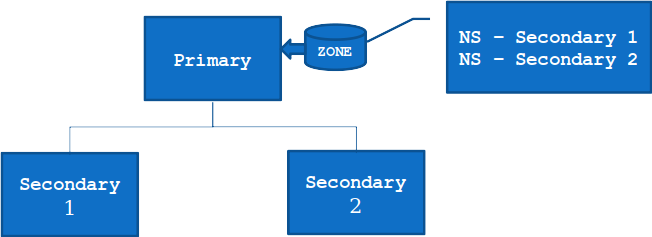
\includegraphics[width=.7\linewidth]{Secondary.png}
    \end{center}
  \end{figure}
\end{frame}

\begin{frame}{Configuring the \texttt{zone}}
  \begin{tcolorbox}[title={\textbf{PERFORMANCE:}}]
    By configuring the \texttt{SOA} record you can control the amount of updating and the time period of caching that is carried out. Tailoring the \texttt{SOA} is a vital part of the \texttt{DNS} architecture and should be carried out based on the profile of a \texttt{zone}'s activity.
  \end{tcolorbox}
  \begin{figure}
    \begin{center}
      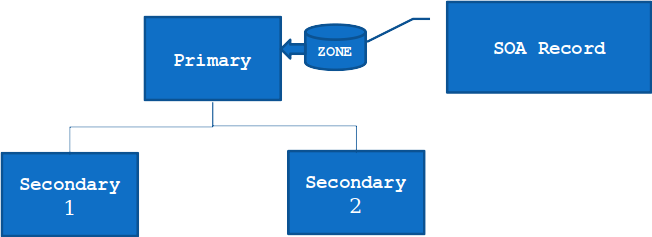
\includegraphics[width=.7\linewidth]{Secondary2.png}
    \end{center}
  \end{figure}
\end{frame}

\begin{frame}[fragile]{\texttt{SOA RR} and \texttt{secondary} servers}
  \begin{itemize}
    \item The \texttt{SOA} record controls the distribution of the \texttt{zone} database and how a \texttt{secondary} refreshes the cached version.
  \end{itemize}
  \begin{tcolorbox}
    \lstset{
      basicstyle=\tiny\ttfamily,
    }
    \begin{lstlisting}
      example.com. IN SOA ns.example.com. hostmaster.example.com. ( 
	        2019091900  ; sn = serial number 
	        172800      ; ref = refresh = 2d 
	        900         ; ret = update retry = 15m 
	        1209600     ; ex = expiry = 2w 
	        3600        ; nx = nxdomain ttl = 1h 
      ) 
    \end{lstlisting}
  \end{tcolorbox}
  \begin{tcolorbox}[title={\textbf{PERFORMANCE:}}]
    \scriptsize \texttt{notify no;} in the \texttt{zone} declaration is used to prevent \texttt{zone} transfers when a \texttt{primary server} is restarted forcing the \texttt{SOA} values to be used by the \texttt{secondary}.\\
    \scriptsize \texttt{notify no;} can also be declared in \texttt{options\{\}} declaration to effect all \texttt{zones}.    
  \end{tcolorbox}
\end{frame}

\begin{frame}{Configuring the Primary \texttt{DNS} for transfers}
  \begin{itemize}
    \item For all the changes to take effect and function correctly you must restart all the \texttt{DNS} servers.
    \item All cached databases files are stored in:-
      \begin{itemize}
        \item \texttt{/var/cache/bind/}
      \end{itemize}
  \end{itemize}
  \begin{tcolorbox}[title={\textbf{NOTE:}}]
    This location is already enabled for \texttt{bind9} to store data, we will cover \texttt{AppArmor} in a moment.
  \end{tcolorbox}
\end{frame}

\begin{frame}{Configuring the Primary \texttt{DNS} for transfers}
  \begin{itemize}
    \item These changes on the \texttt{secondary DNS} server will result in entries in the system log showing that the operation has been carried out.
      \begin{itemize}
        \item \texttt{/var/log/syslog}
      \end{itemize}
    \item You can view the end of the \texttt{syslog} using the \texttt{tail} command.
      \begin{itemize}
        \item e.g. \texttt{\$sudo tail -25 /var/log/syslog}
      \end{itemize}
  \end{itemize}
\end{frame}

\section{Management}
\subsection{Managing the \texttt{DNS}}
\begin{frame}{Forcing Primary \texttt{DNS} updates}
  \begin{itemize}
    \item Changes can be made on an ad-hoc basis to the \texttt{Primary}'s \texttt{zone}s.
    \item Given time (\texttt{SOA} or \texttt{notified yes;}) the \texttt{secondary} servers will retrieve any changes that are made.
    \item You may on occasions need to force a refresh of a \texttt{Secondary DNS} to update a \texttt{zone} cache.
    \item One of the many utilities you have to manage your \texttt{DNS} is the \texttt{rndc}.
      \begin{itemize}
        \item e.g. \texttt{\$sudo rndc refresh <zone>}
      \end{itemize}
  \end{itemize}
\end{frame}

\subsection{Query Logging}
\begin{frame}{Logging \texttt{DNS} activity}
  \begin{itemize}
    \item A common practice in identifying issues with \texttt{DNS} infrastructures is to enable \texttt{DNS} logging.
    \item Logging is also used as a mechanism to determine the activity of a \texttt{DNS} architecture.
    \item However:
      \begin{itemize}
        \item What have the users been looking at (Big Brother!!!!)
        \item This information can be used to block unwanted sites in a firewall.
      \end{itemize}
  \end{itemize}
\end{frame}

\begin{frame}{Logging \texttt{DNS} activity}
  \begin{itemize}
    \item There are many options that can be used but the two primary logging directives that we are interested in are:-
      \begin{itemize}
        \item \texttt{Channel} - The log file location
        \item \texttt{Category} - What information is logged
      \end{itemize}
  \end{itemize}
\end{frame}

\begin{frame}[fragile]{Logging \texttt{DNS} activity}
  \begin{itemize}
    \item Logging is enabled in \texttt{/etc/bind/named.conf.local}
  \end{itemize}
  \begin{tcolorbox}
    \lstset{
      basicstyle=\tiny\ttfamily,
    }
    \begin{lstlisting}
      logging {
	      channel query.log {
	          file "/var/log/query.log";
	          severity debug 3;
	      };
	      category queries { query.log; };
      };
    \end{lstlisting}
  \end{tcolorbox}
\end{frame}

\begin{frame}{Create the log file}
  \begin{itemize}
    \item Since the \texttt{named daemon} runs as the \texttt{bind} user the log file must be created and the ownership changed.
      \begin{itemize}
        \item \texttt{\$sudo touch /var/log/query.log }
        \item \texttt{\$sudo chown bind /var/log/query.log}
      \end{itemize}
  \end{itemize}
  \begin{tcolorbox}[title={\textbf{NOTE:}}]
      \begin{center}
        You could just use the \texttt{/var/log/named/} folder (\texttt{bind9} has \texttt{R/W} privileges by default) but then we wouldn't get to play with \texttt{AppArmor}?        
      \end{center}
  \end{tcolorbox}
\end{frame}

\begin{frame}{Create the log file}
  \begin{itemize}
    \item Before the \texttt{named daemon} can write to the new log file the \texttt{AppArmor} profile must be updated.
      \begin{itemize}
        \item \texttt{AppArmor} is a process manager that controls access to system resources.
      \end{itemize}
    \item To configure the \texttt{AppArmor} service you need to edit the \texttt{AppArmor config} file.
  \end{itemize}
  \begin{tcolorbox}
      \begin{center}
        \texttt{/etc/apparmor.d/usr.sbin.named}
      \end{center}
  \end{tcolorbox}
\end{frame}

\begin{frame}{Create the log file}
  \begin{itemize}
    \item The config file needs to have the new log file added to it.
      \begin{itemize}
        \item \texttt{/var/log/query.log rw,}
      \end{itemize}
    \item Next reload the profile \texttt{AppArmor} changes:
      \begin{itemize}
        \item \scriptsize\texttt{\$sudo apparmor\_parser -r /etc/apparmor.d/usr.sbin.named}
      \end{itemize}
    \item Finally, restart the \texttt{bind9} daemon for logging to begin.
    \item Don't forget to comment out the logging and restart \texttt{bind9} to stop logging.
  \end{itemize}
  \begin{tcolorbox}[title={\textbf{CONSIDER:}}]
    \begin{center}
      When and where would you use logging?
    \end{center}
\end{tcolorbox}
\end{frame}

\section*{Conclusion}
\begin{frame}{Conclusion}
  \begin{itemize}
    \item What is a \texttt{secondary DNS} Server?
    \item What does and \texttt{DNS} infrastructure provide when it includes secondary servers?
    \item How do you log \texttt{DNS} transactions?
    \item What is the purpose of logging transactions on a \texttt{DNS} server?
  \end{itemize}
\end{frame}

\end{document}


